\documentclass[border=10pt]{standalone}
\usepackage[svgnames]{xcolor}
\usepackage{amsmath}
\usepackage{pgfplots}
\pgfplotsset{compat=newest}
\usepackage[sfdefault]{FiraSans}
\usepackage{FiraMono}
\renewcommand*\familydefault{\sfdefault}
\begin{document}
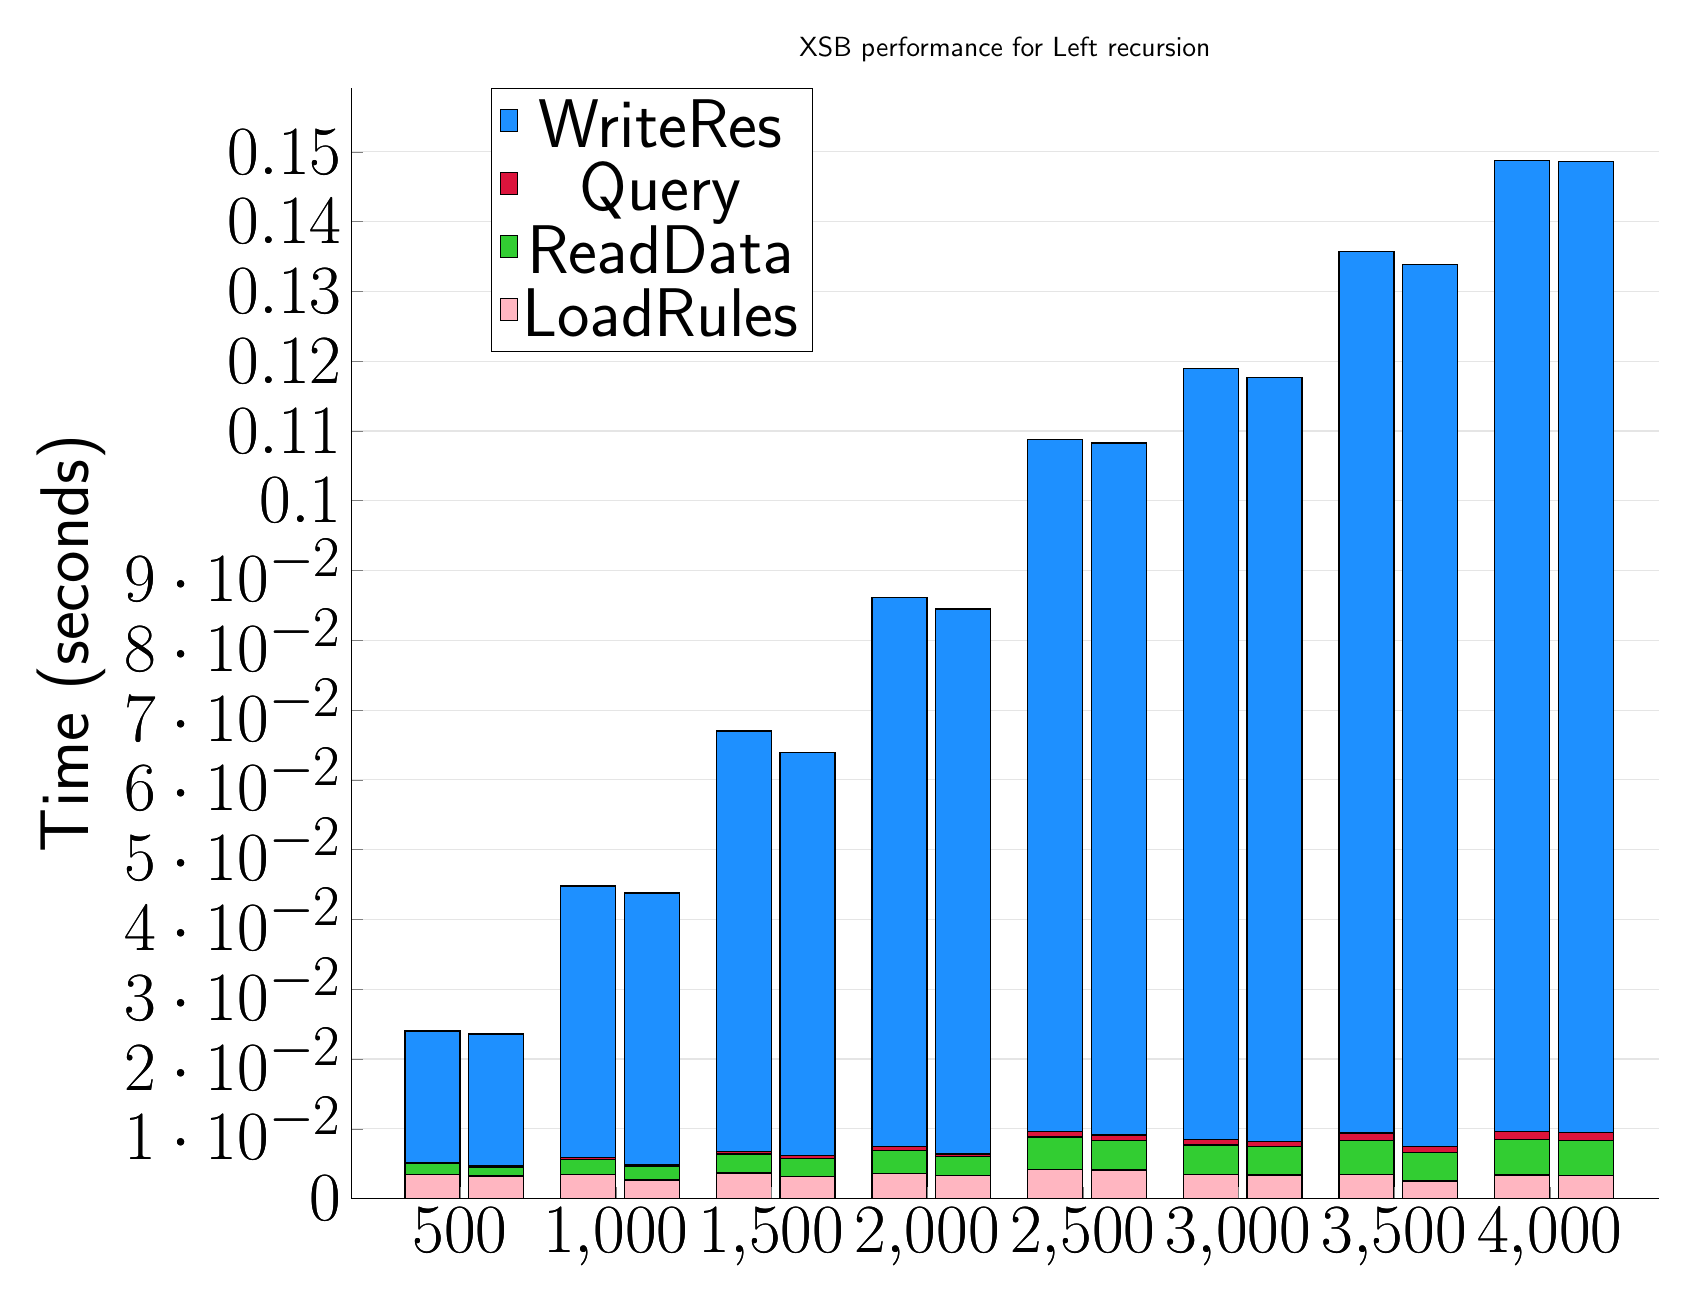
\begin{tikzpicture}
\begin{axis}[
   ybar stacked,
   title={XSB performance for Left recursion},
   bar shift=-10pt,
   width=1.5\textwidth,
   bar width=0.7cm,
   ymajorgrids, tick align=inside,
   major grid style={draw=gray!20},
   xtick=data,
   ymin=0, ymax=0.15917342821757002,
   axis x line*=bottom,
   axis y line*=left,
   enlarge x limits=0.1,
   legend style={
       at={(0.23, 1)},
       anchor=north,
       legend columns=1,
       font=\Huge,
   },
   ylabel={Time (seconds)},
   label style={font=\Huge},
   tick label style={font=\Huge},
]
\addlegendimage{fill=DodgerBlue, draw=black, line width=0.2pt}
\addlegendentry{WriteRes}
\addlegendimage{fill=Crimson, draw=black, line width=0.2pt}
\addlegendentry{Query}
\addlegendimage{fill=LimeGreen, draw=black, line width=0.2pt}
\addlegendentry{ReadData}
\addlegendimage{fill=LightPink, draw=black, line width=0.2pt}
\addlegendentry{LoadRules}
\addplot +[fill=LightPink, draw=black, line width=0.5pt] coordinates {
    (500, 0.00343791643778483)
    (1000, 0.00346088409423828)
    (1500, 0.00364120801289876)
    (2000, 0.0036293665568033866)
    (2500, 0.004126707712809243)
    (3000, 0.003422657648722333)
    (3500, 0.00344705581665039)
    (4000, 0.0033532778422037768)
};
\addplot +[fill=LimeGreen, draw=black, line width=0.5pt] coordinates {
    (500, 0.0015470186869303364)
    (1000, 0.00213940938313802)
    (1500, 0.0027294158935546897)
    (2000, 0.0032525857289632167)
    (2500, 0.004685242970784503)
    (3000, 0.004272619883219403)
    (3500, 0.004915316899617513)
    (4000, 0.0051390329996744795)
};
\addplot +[fill=Crimson, draw=black, line width=0.5pt] coordinates {
    (500, 0.00014162063598632834)
    (1000, 0.00027195612589518236)
    (1500, 0.00041500727335611965)
    (2000, 0.0006213188171386717)
    (2500, 0.0007877349853515624)
    (3000, 0.0007656415303548177)
    (3500, 0.0010236899058024102)
    (4000, 0.00110801060994466)
};
\addplot +[fill=DodgerBlue, draw=black, line width=0.5pt] coordinates {
    (500, 0.018899122873942038)
    (1000, 0.03890371322631835)
    (1500, 0.060213963190714516)
    (2000, 0.07866366704305013)
    (2500, 0.0991768836975096)
    (3000, 0.11049461364746117)
    (3500, 0.1263310909271239)
    (4000, 0.13917342821757003)
};
\end{axis}
\begin{axis}[
   ybar stacked,
   bar shift=13pt,
   width=1.5\textwidth,
   bar width=0.7cm,
   ymajorgrids, tick align=inside,
   major grid style={draw=none},
   xtick=data,
   ymin=0, ymax=0.15917342821757002,
   axis x line*=none,
   axis y line*=none,
   enlarge x limits=0.1,
   label style={font=\Huge},
   tick label style={font=\Huge},
]
\addplot +[fill=LightPink, draw=black, line width=0.5pt] coordinates {
    (500, 0.0032156666666666666)
    (1000, 0.0026676666666666667)
    (1500, 0.0031873333333333333)
    (2000, 0.0032736666666666665)
    (2500, 0.0041080000000000005)
    (3000, 0.003396)
    (3500, 0.002521)
    (4000, 0.003336)
};
\addplot +[fill=LimeGreen, draw=black, line width=0.5pt] coordinates {
    (500, 0.001319666666666667)
    (1000, 0.001983333333333333)
    (1500, 0.002572666666666667)
    (2000, 0.0027886666666666667)
    (2500, 0.004228)
    (3000, 0.004048)
    (3500, 0.0040876666666666665)
    (4000, 0.005007999999999999)
};
\addplot +[fill=Crimson, draw=black, line width=0.5pt] coordinates {
    (500, 0.000133000000000001)
    (1000, 0.000271999999999999)
    (1500, 0.00041433333333333366)
    (2000, 0.00034633333333333266)
    (2500, 0.0007863333333333333)
    (3000, 0.000765333333333332)
    (3500, 0.0008849999999999986)
    (4000, 0.0011076666666666667)
};
\addplot +[fill=DodgerBlue, draw=black, line width=0.5pt] coordinates {
    (500, 0.018907)
    (1000, 0.038862)
    (1500, 0.05775566666666667)
    (2000, 0.07807866666666667)
    (2500, 0.09913633333333333)
    (3000, 0.10946766666666667)
    (3500, 0.12635366666666667)
    (4000, 0.13916366666666666)
};
\end{axis}
\end{tikzpicture}

\end{document}
